%
% File XCS229ii_final_paper.tex
%

\documentclass[11pt,a4paper]{article}
\usepackage[hyperref]{acl2020}
\usepackage{times}
\usepackage{latexsym}
\usepackage{graphicx}
\usepackage{amsmath}
\renewcommand{\UrlFont}{\ttfamily\small}

% This is not strictly necessary, and may be commented out,
% but it will improve the layout of the manuscript,
% and will typically save some space.
\usepackage{microtype}

\aclfinalcopy % Uncomment this line for the final submission
%\def\aclpaperid{***} %  Enter the acl Paper ID here

%\setlength\titlebox{5cm}
% You can expand the titlebox if you need extra space
% to show all the authors. Please do not make the titlebox
% smaller than 5cm (the original size); we will check this
% in the camera-ready version and ask you to change it back.

\newcommand\BibTeX{B\textsc{ib}\TeX}

\title{Melanoma Segmentation using Convolutional and Transformer based Deep Neural Networks}

\author{
  Akshay Agarwal \\
  \texttt{aa2657@cornell.edu} \\
  \And
  Manish Das \\
  \texttt{z.manishdas@gmail.com} \\
  \AND
  Jaro Habr \\
  \texttt{jaro.habr@gmail.com} \\
  \And
  Parag Kanade \\
  \texttt{p\_kanade@yahoo.com} \\
}

\date{}

\begin{document}
\maketitle

\begin{abstract}

Melanoma is the most dangerous and deadliest skin cancer type causing over \$8 billion in health care costs annually in the United States alone. In this work we investigate the application of state-of-the-art computer vision Transformer based architectures on the task of semantic skin lesion segmentation. We compare the Medical Transformer and TransUNet models with the widely used U-Net, a convolutional neural network (CNN) specifically developed for medical image segmentation, to study their performance on the melanoma segmentation challenge dataset published by the International Skin Imaging Collaboration (ISIC). We show that vision Transformers achieve better results than their established CNN based counterparts in some aspects as expressed by the specificity metric, perform comparably well as measured by accuracy or Dice Coefficient, but show evident weaknesses as revealed by the threshold Jaccard Index metric. It is worth noticing that the performance gains are often minimal and come with higher computational cost. Furthermore, our work shows that an appropriate image pre-processing and data augmentation play a crucial role in medical segmentation tasks as data is often scarce and shows varying quality characteristics.

% \begin{itemize}
%   \item One paragraph summary of the entire paper
%   \item include the results and the implications of those results (i.e. social, business, etc.)
% \end{itemize}

\end{abstract}
\section{Introduction}

\begin{itemize}
  \item Describe the topic under investigation.
  \item Summarize prior research in this area \citep{vaswani-2017-attention}.
  \item Identification of unresolved issues that your current paper will address.
  \item Provides a overview of the paper and sections to follow.
\end{itemize}

\section{Methods}

\subsection{Dataset}
We use the melanoma segmentation dataset as published in the 2018 Lesion Boundary Segmentation Challenge by the International Skin Imaging Collaboration (ISIC) \citep{isic-2018-segmentation}. The dataset comprises dermatoscopic images with their corresponding ground truth segmentation masks \citep{ensambles-2016-codella}.

\par
The \emph{lesion} images were acquired by different dermatoscope types from several institutions, taken from all anatomic sites and from a historical sample of patients presented for skin cancer screening. Every image contains exactly one primary lesion. The distribution of disease states represent a modified "real world" setting (over-representation of malignancies) containing more benign lesions than malignant. All lesion images are named using the scheme ISIC\_\textless{image}\_id\textgreater{.jpg} with the \textless{image}\_id\textgreater{} being a 7-digit identifier \citep{isic-2018-segmentation}.

\par
The ground truth is represented by binary segmentation masks which indicate the location of the primary skin lesion within each input image. Mask images follow a similar naming scheme, namely  ISIC\_\textless{image\_id}\textgreater{\_segmentation.png}, and have the exact same dimensions as the lesion images. The masks are represented by a single-channel 8-bit continuous region, where each pixel is either 0 (background - area outside of the primary lesion) or 255 (foreground - area inside the primary lesion). The ground truth images were obtained using several techniques (e.g. fully automated algorithm; manual polygon tracing by human expert annotators), but all data were reviewed by practicing dermatologists with expertise in dermoscopy \citep{isic-2018-segmentation,ensambles-2016-codella}.

\par
The dataset is divided into train, validation and test sets with 2’594, 100 and 1’000 images respectively. The train and validation datasets contain the exact same number of ground truth segmentation mask images whereas the test dataset does not. The test dataset is used for the final evaluation of the challenge submission and hence does not contain any segmentation masks. Figure \ref{datasets} shows image size distribution per dataset.

\begin{figure}[ht]
\centering
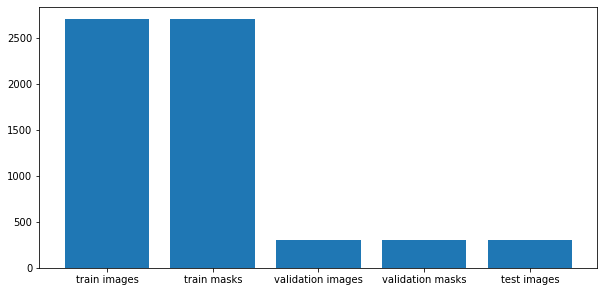
\includegraphics[width=\columnwidth]{assets/datasets.png}
\caption[Datasets]
{Image distribution in the train, validation and test datasets (ISIC 2018 segmentation challenge).}
\label{datasets}
\end{figure}

The images in each dataset show a spectrum of variations in terms of quality (e.g. sharpness, lighting conditions, coloring etc.) and added noise (e.g. hair, rulers, bubbles etc.). Furthermore, the resolution of the images varies significantly. The \emph{train} dataset has 206 different dimensions, ranging from a resolution of 540 x 722 pixels to 4'499 x 6'748 pixels. The \emph{validation} dataset has 21 different resolutions, ranging from 480 x 640 pixels to 4'461 x 6'641 pixels. Lastly, the \emph{test} dataset has 114 different resolutions, ranging from 480 x 640 pixels to 4'519 x 6'808 pixels. Figure \ref{lesion_images} shows three examples of lesion images and their corresponding binary segmentation masks.

\begin{figure}[ht]
\centering
\includegraphics[width=\columnwidth]{assets/lesion_images.pdf}
\caption[Lesion Images]
{Three lesion images with different noise on the top with their corresponding binary masks at the bottoms.}
\label{lesion_images}
\end{figure}


% \begin{itemize}
%   \item Define your task in a clear, concise manner
%   \item Formally describe each model under investigation. Include your baseline and experimental models at minimum.
%   \item For each model, describe its infrastructure and assumptions (if applicable).
% \end{itemize}

\section{Results}

In this subsection we first describe the metrics used to evaluate the performance of the models on the skin lesion segmentation task. We then present the experimental environment setup and show the final results.

\subsection{Metrics}

Image segmentation models are mostly evaluated on the basis of how accurately they can predict each pixel. The prediction of the pixels can fall into one of four categories: true positive (TP), true negative (TN) or false positive (FP) and false negative (FN) respectively. The model’s performance is determined by the nature of its prediction and the aforementioned category it belongs to and the computed metrics derived therefrom.

The 2018 lesion segmentation challenge defines the \emph{Threshold Jaccard Index}, averaged over all images in the dataset, as the primary evaluation criteria where the threshold is set to 0.65 \citep{challenge-2018-codella}. The \emph{Jaccard Index}, also called Intersection over Union (IoU), is a method to quantify the percentage of overlap between the target mask (A) and our prediction output (B). It is formally defined as

\begin{equation}
  J(A, B) = \frac{|A \cup B|}{|A \cap B|}
\end{equation}

The Threshold Jaccard Index can then be calculated as

\begin{equation}
  TJ(A, B) = \begin{cases}
      J(A, B), & \text{if}\ J(A, B) \geq{0.65} \\
      0, & \text{otherwise}
    \end{cases}
\end{equation}

The Jaccard Index metric is closely related to the \emph{Dice Coefficient} which is often used as a loss function during training. We use the Dice Coefficient to calculate the area of overlap between the target mask and the predicted mask, defined as

\begin{equation}
  Dice = \frac{2TP}{2TP + FN + FP}
\end{equation}

Furthermore, \emph{accuracy} helps us to track the ratio between correctly predicted pixels over all pixels. For a given prediction, accuracy is defined as

\begin{equation}
  Accuracy = \frac{TP + TN}{TP + FP + TN + FN}
\end{equation}

Finally, \emph{sensitivity} measures the proportion of the correctly identified positives and is   calculated as

\begin{equation}
  Sensitivity = \frac{TP}{TP + FN}
\end{equation}

\emph{Specificity} tells us the proportion of the correctly identified negatives  and can be calculated as

\begin{equation}
  Specificity = \frac{TN}{TN + FP}
\end{equation}


\subsection{Experiments}

\subsubsection{Training Environment Setup}

All experiments were conducted using the same VM setup running Linux 18.04.1-Ubuntu (x86\_64). The underlying hardware contained 54 GiB physical memory, 64-bits Intel(R) Xeon(R) CPU E5-2690 v3 (2.60GHz) and NVIDIA Tesla K80 (8GK210GL, rev a1) GPU with 12 GiB physical memory.

\subsubsection{Approach}

We designed and ran 27 experiments in total. We used the following three machine learning frameworks as our experiment design guide:

\textbf{Ablative Analysis}: In order to determine the optimal image size for each model given the time and resources constraints, we performed ablation studies with input resolutions of 512x512 pixels, 2556x256 pixels, 192x256 pixels and 128x128 pixels. We also study the impact of transfer learning on the selected model architecture by adding or removing encoder weights pretrained on ImageNet. Furthermore, we study the effect of different encoder backbones in our encoder-decoder architectures.

\textbf{Approximation and estimation error}: We use the accuracy metrics to measure the performance of the models during training and inference time. We test different data preprocessing techniques like removing or adding hair to measure how much error is attributable to each method.

\textbf{Bias-variance diagnostic}: We use various regularization techniques like early stopping to understand the bias-variance trade-off and to prevent the models from overfitting in order to generalize well on unseen data. For final performance comparison, we report all previously defined metrics on an unseen test dataset.

\par
Table \ref{table:experiments} shows an overview over all experiment setups.

\begin{table*}[ht]
  \centering
  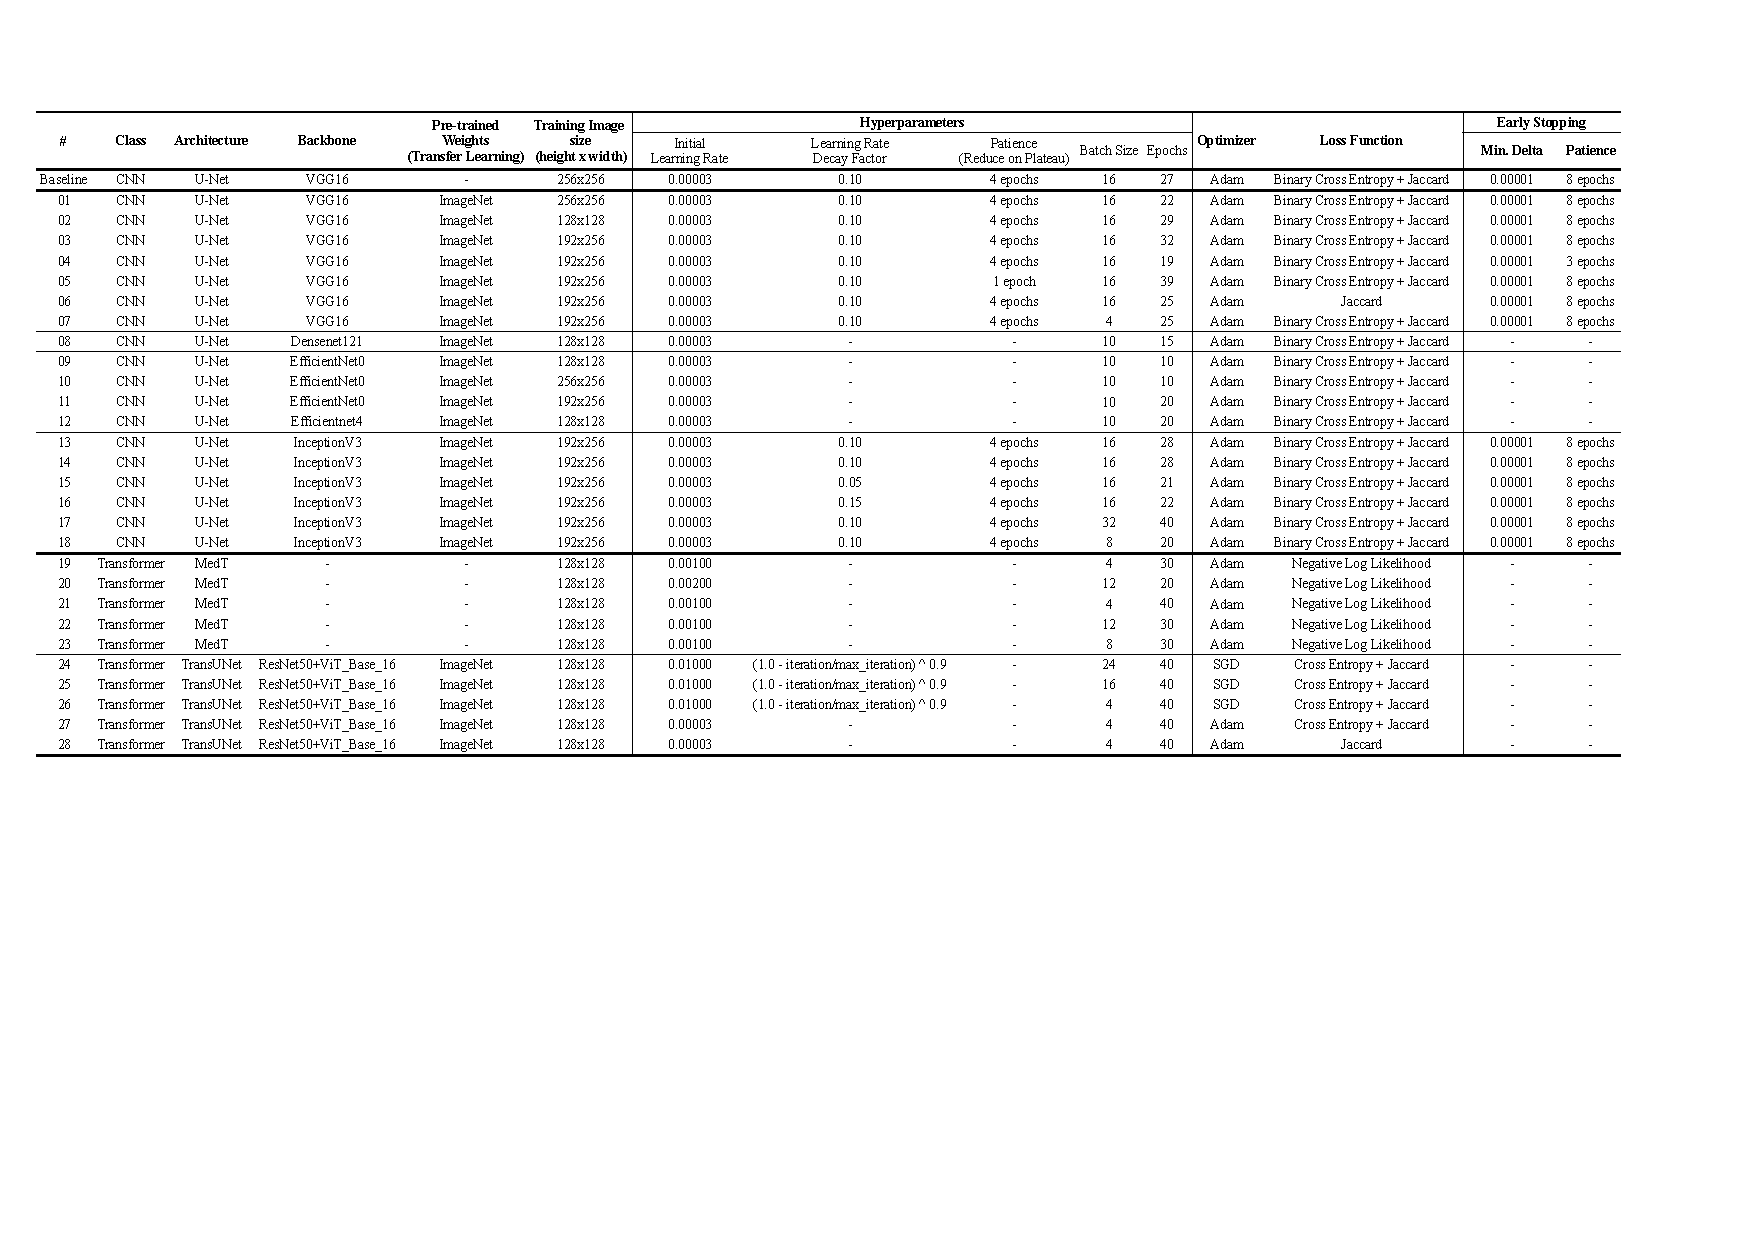
\includegraphics[width=\textwidth]{assets/experiments.pdf}
  \caption[Experiments]{Experimental model configurations with hyperparameter settings, optimizer, loss function and early stopping setup. First row corresponds to the baseline model.}
  \label{table:experiments}
\end{table*}

\par
Table \ref{table:results} summarizes all experiment results.

\begin{table*}[ht]
  \centering
  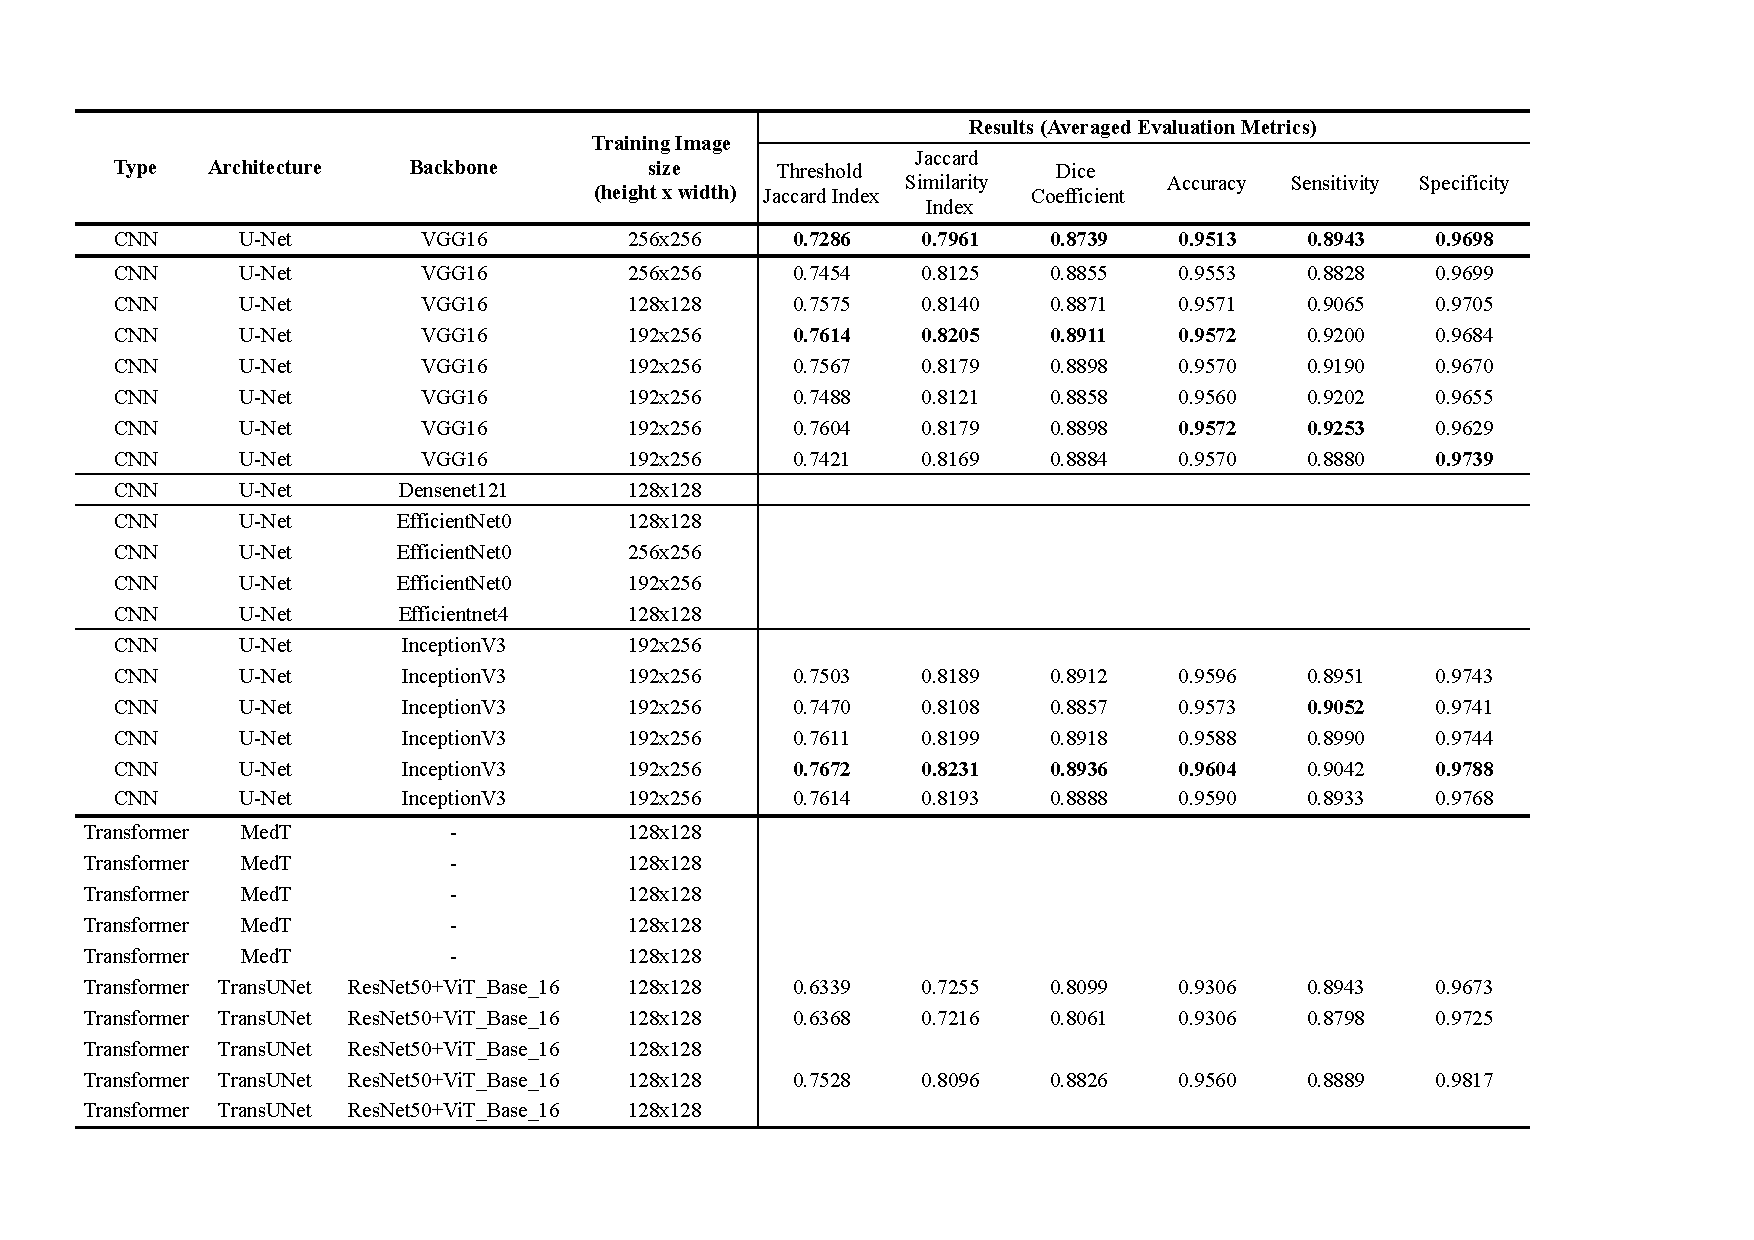
\includegraphics[width=\textwidth]{assets/results.pdf}
  \caption[Results]{Model flavors with corresponding type, architecture, input image sizes and final results as reported on unseen test dataset. First row corresponds to the baseline model.}
  \label{table:results}
\end{table*}

% \begin{itemize}
%   \item Describe all Machine Learning Theory techniques used to evaluate the success of the model.
%   \item Describe how results compare to previous research.
% \end{itemize}

\section{Discussion}

Skin cancer is the most common form of cancer in the United States, with the annual cost exceeding \$8 billion. Melanoma, a type of skin cancer, is the deadliest form. When detected early, the 5-year survival rate can go up to 99\% compared to a delayed diagnosis which causes the survival rate to dramatically drop to 23\% \citep{challenge-2018-codella}.

\par
The contribution of this work is two-fold: First, given the latest developments in computer vision and especially in semantic image segmentation, this work is one of the first to study the impact and performance of Transformer based models \citep{transformers-2020-dosovitskiy} on the specific task of skin lesion segmentation based on the ISIC 2018 challenge \citep{isic-2018-segmentation}. Second, we extend the work of \citep{medical_transformer-2021-valanarasu} and \citep{transunet-2021-chen} by applying their ideas with slight adaptations to a different medical domain and hence extending the knowledge base of the MedT and TransUNet architectures.

\par
Although we weren’t able to show an overall better performance of the Transformer based architecture compared to CNN based architectures as presented by the authors of the original papers for the specific task of skin lesion segmentation, we showed that Transformer based models are superior to CNN based models as measured by some specific metrics like Sensitivity as well as comparable in other metrics like accuracy or Dice coefficient.

\par
Due to time and computational resources constraints, we were able to perform only a subset of the possible and identified experiments. An obvious direction for future work would be to cover more different architectural compositions for both model classes, accompanied by a variation along a defined  hyperparameter space.

\par
As image pre-processing and resizing was one of the main challenges in the project, we might explore different ways of image resizing and augmentation. Ultimately, we would like to use a machine with a bigger GPU so that we can increase the minimum image resolution size required for training. This might help increase the detail level of the predicted mask as less compression would be applied to the input images. We can also expand the segmentation task to melanoma classification in order to build an end-to-end system that could be used for helping diagnosing melanoma using a smartphone.


% \begin{itemize}
%   \item Describe the significance of your results and how those results address the topic under investigation.
%   \item Describe ways of expanding upon the implications of your findings.
%   \item Limitations and directions of future research.
% \end{itemize}

\section{Future Work}

Many different tests, architecture and experiments have been left for the future due to lack of time. We can try more CNN and Transformers based models with varying  hyperparameters. As image preprocessing and resizing was one of the main challenges in the project, we might explore different ways of image resizing and augmentation. Ultimately we would like to use a machine with a bigger GPU so that we can increase the minimum image resolution size required for training. We can also expand the segmentation task to melanoma classification to build an end-to-end system.

\section*{Acknowledgments}

We thank Prof. Andrew Ng, our course facilitator Cécile Longé and the staff of XCS229ii for their guidance throughout this project.


\bibliography{references}
\bibliographystyle{acl_natbib}

\appendix
\clearpage
\section{Appendix}
\label{sec:appendix}

\begin{figure}[htb!]
  \centering
  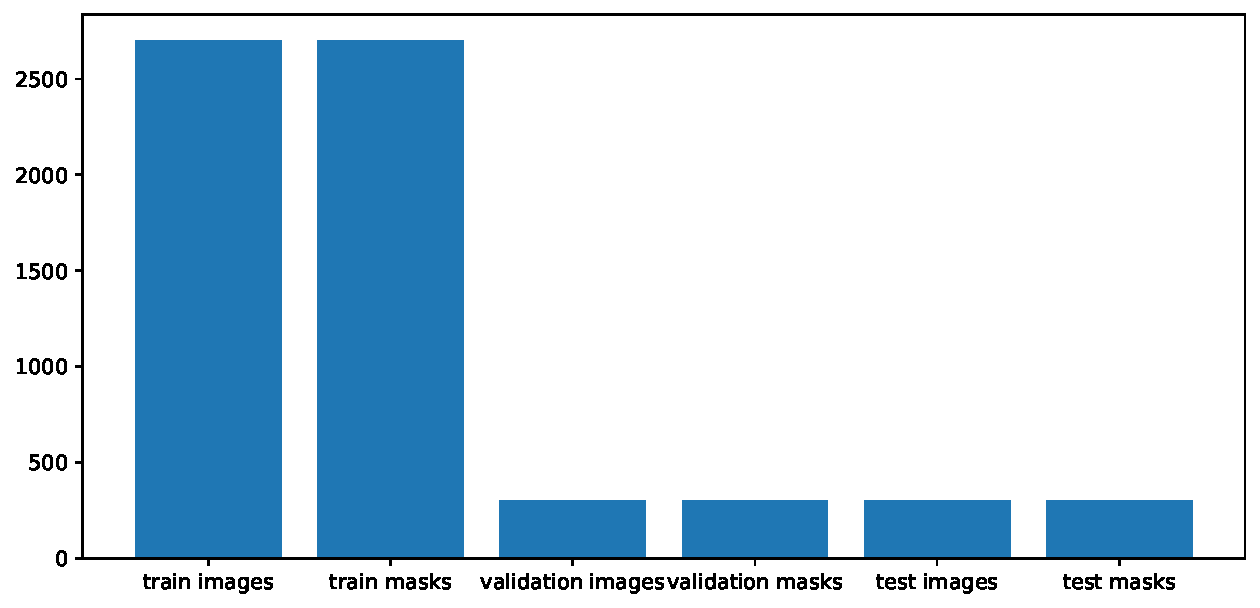
\includegraphics[width=\textwidth]{assets/datasets.pdf}
  \caption{Datasets}
  {Image distribution in the train, validation and test datasets (ISIC 2018 segmentation challenge).}
  \label{datasets}
\end{figure}

\clearpage

\begin{figure}[htb!]
  \centering
  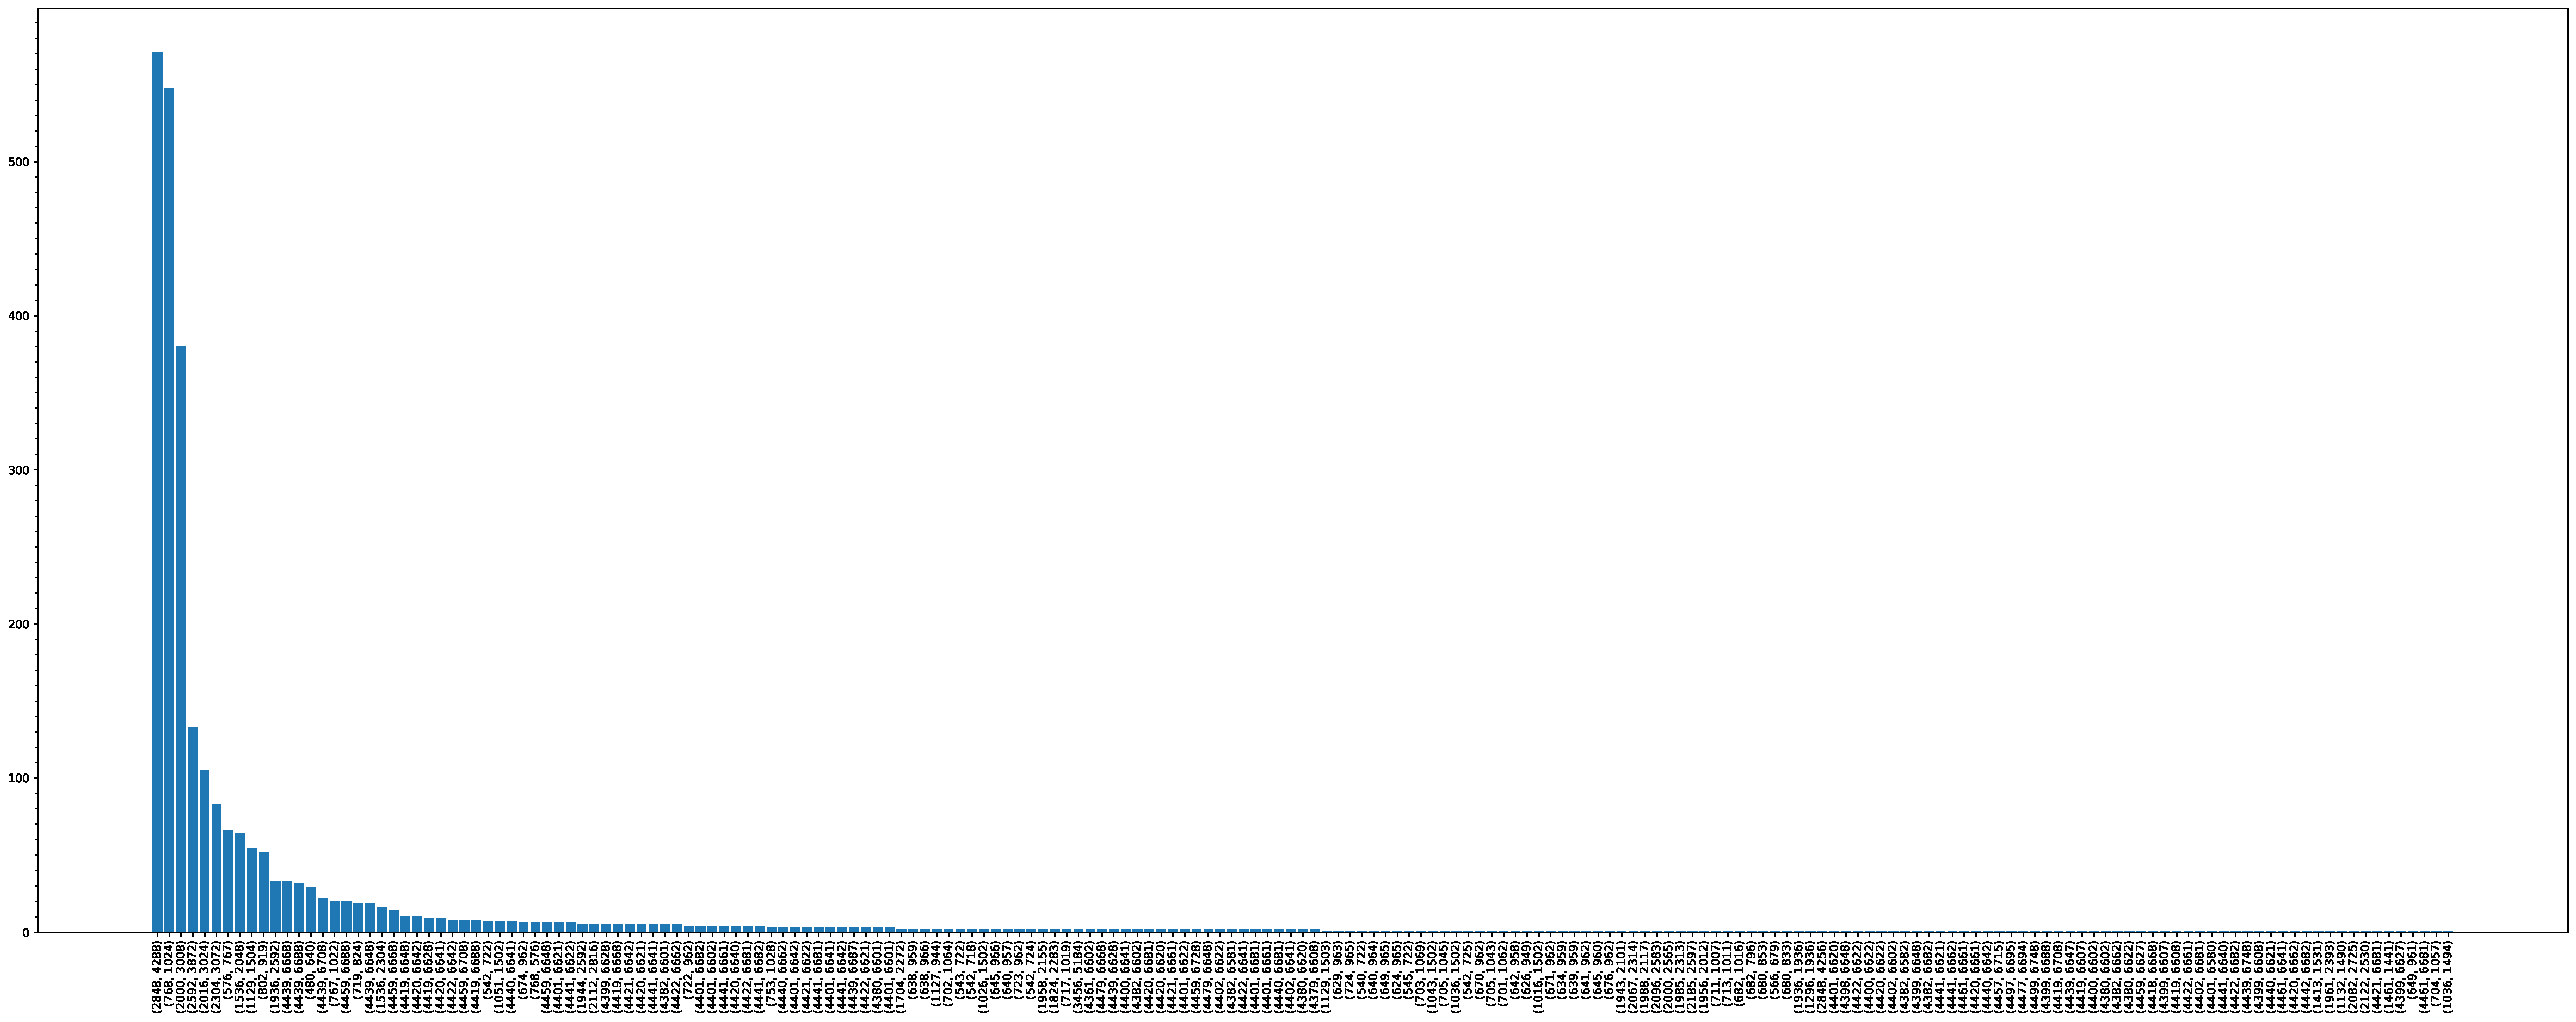
\includegraphics[width=\textwidth]{assets/train_image_resolutions.pdf}
  \caption{Train image resolution distribution.}
  \label{figure:1}
\end{figure}

\begin{figure}[htb!]
  \centering
  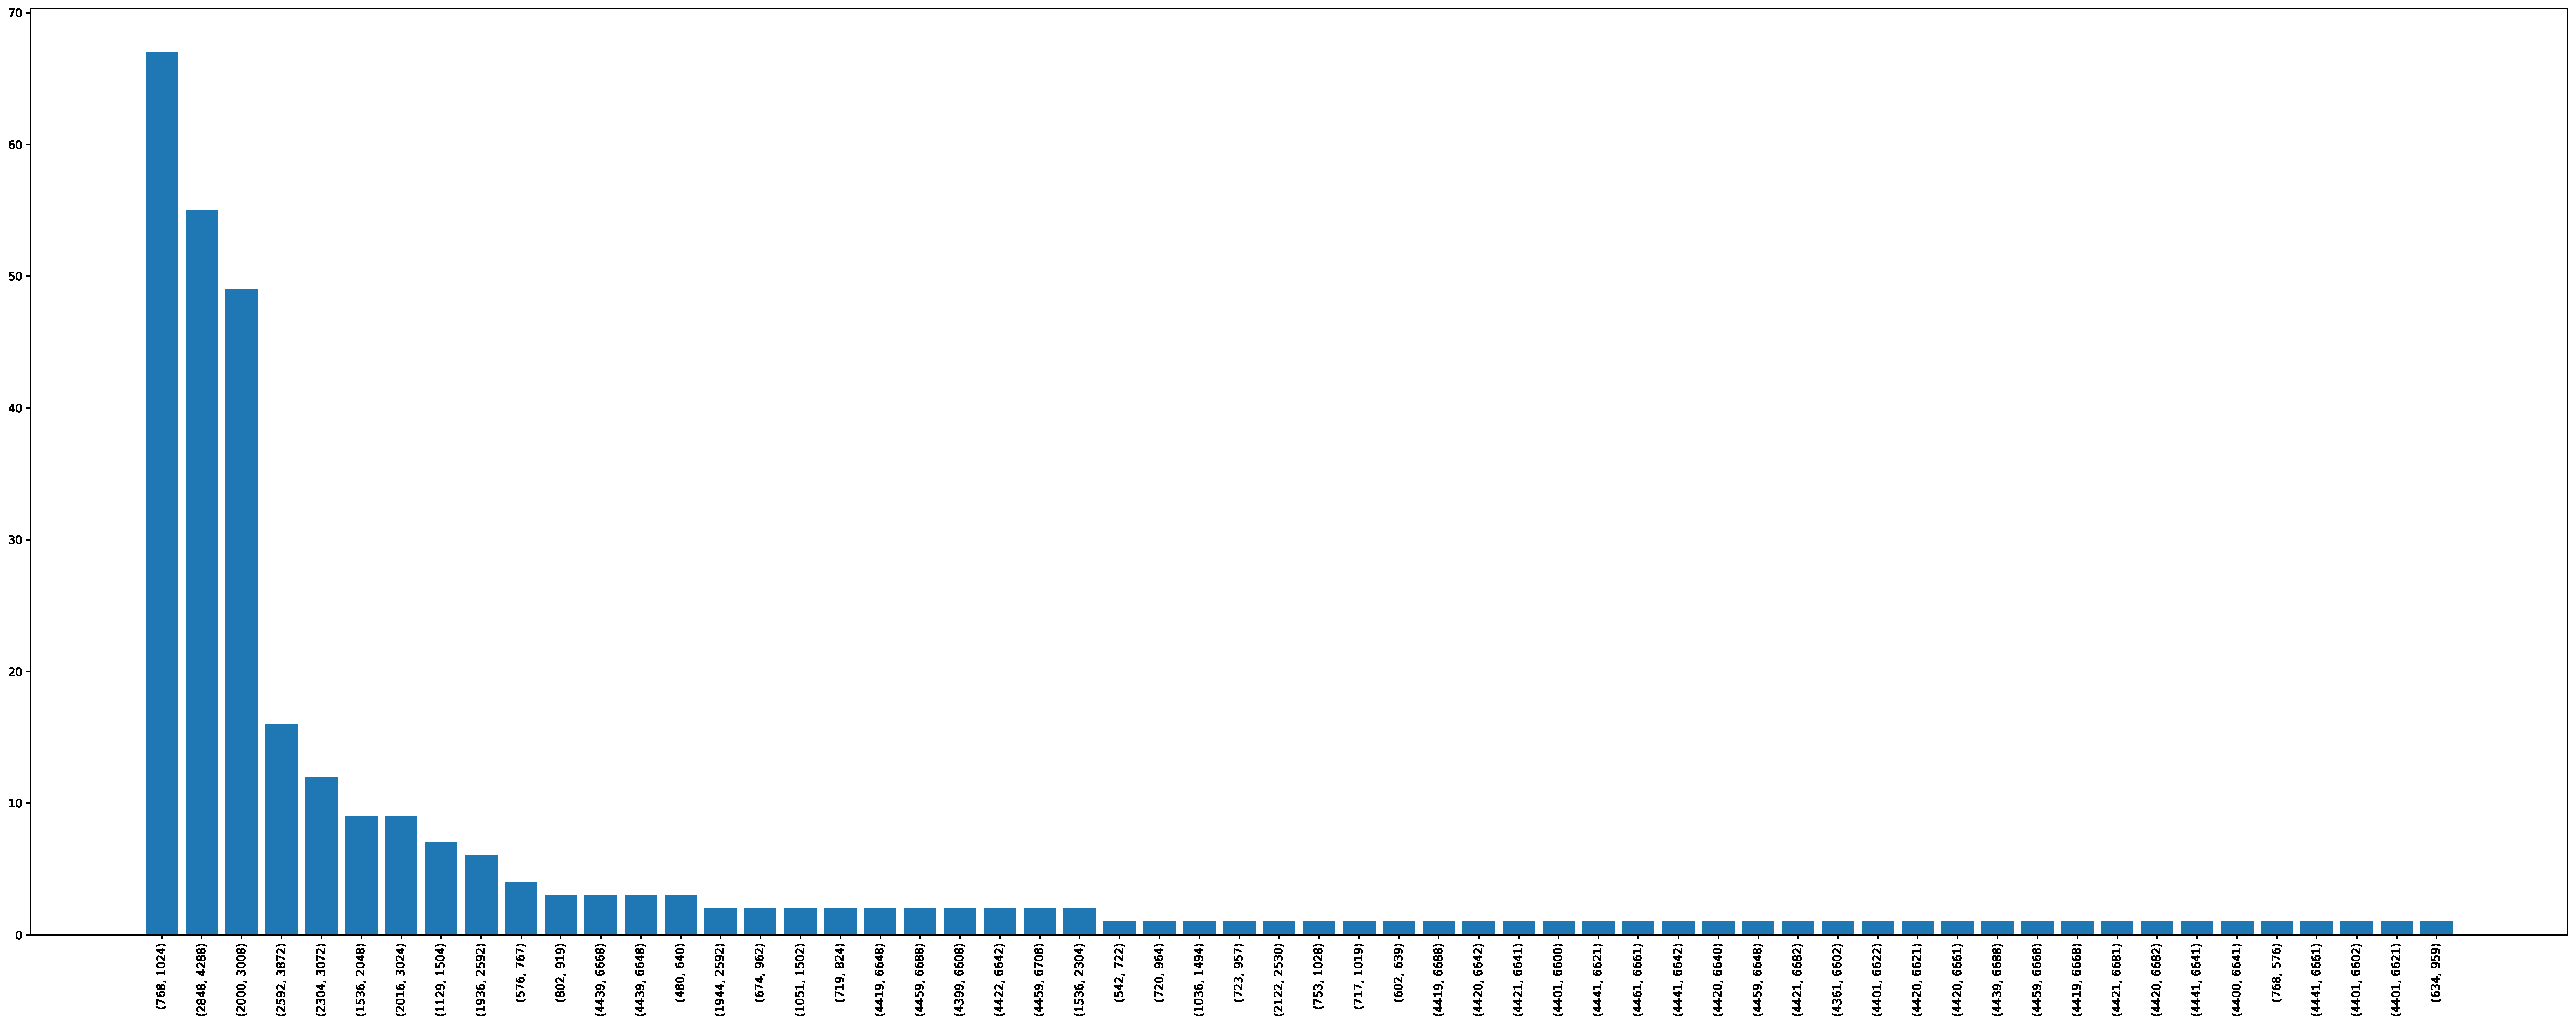
\includegraphics[width=\textwidth]{assets/valid_image_resolutions.pdf}
  \caption{Validation image resolution distribution.}
  \label{figure:2}
\end{figure}

\begin{figure}[htb!]
  \centering
  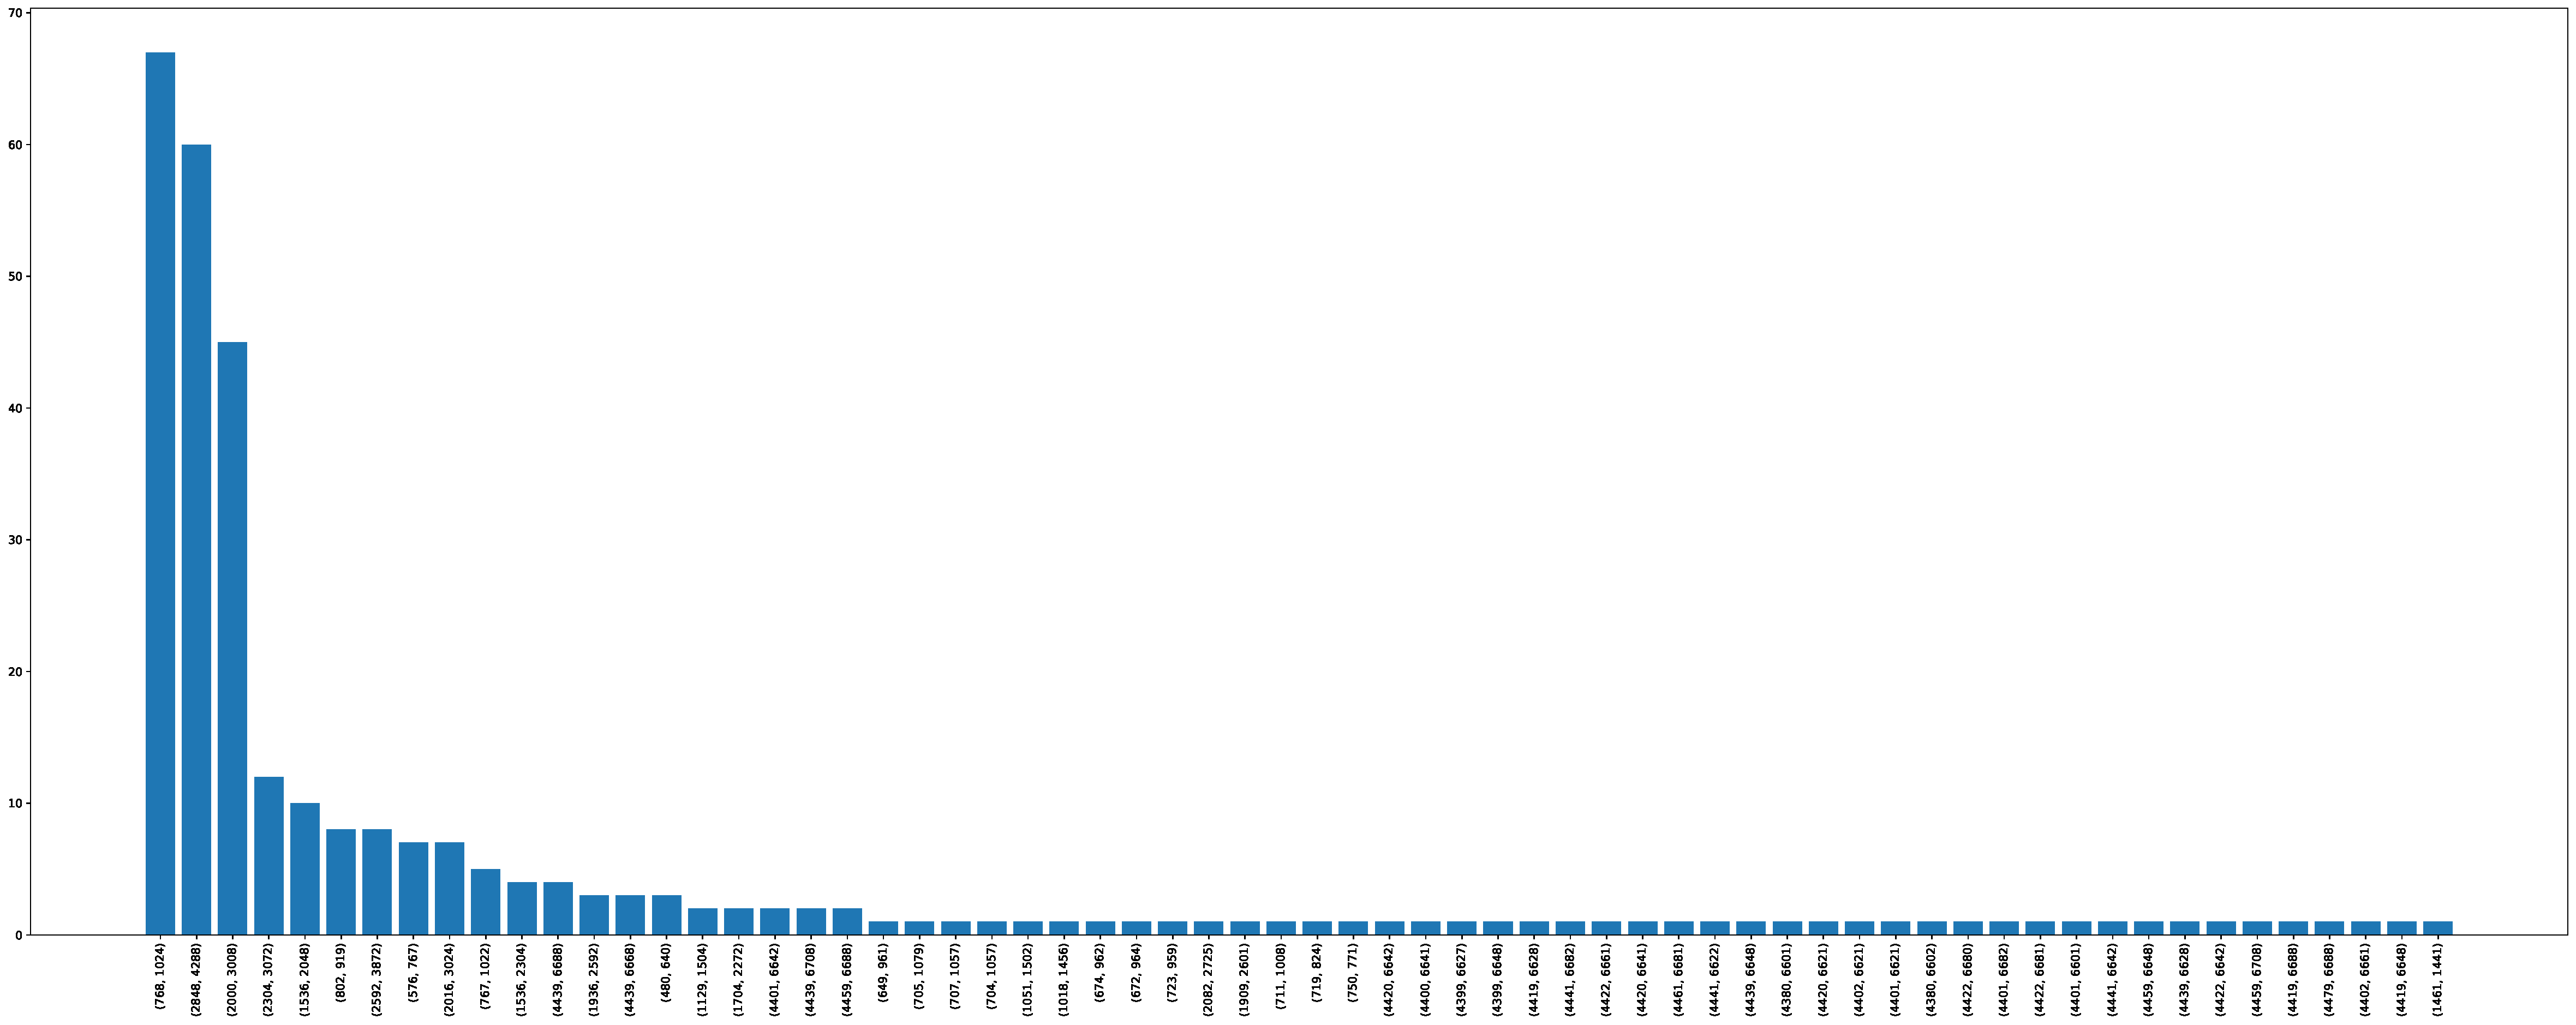
\includegraphics[width=\textwidth]{assets/test_image_resolutions.pdf}
  \caption{Test image resolution distribution.}
  \label{figure:3}
\end{figure}

% \clearpage

% \begin{figure}[ht]
%   \centering
%   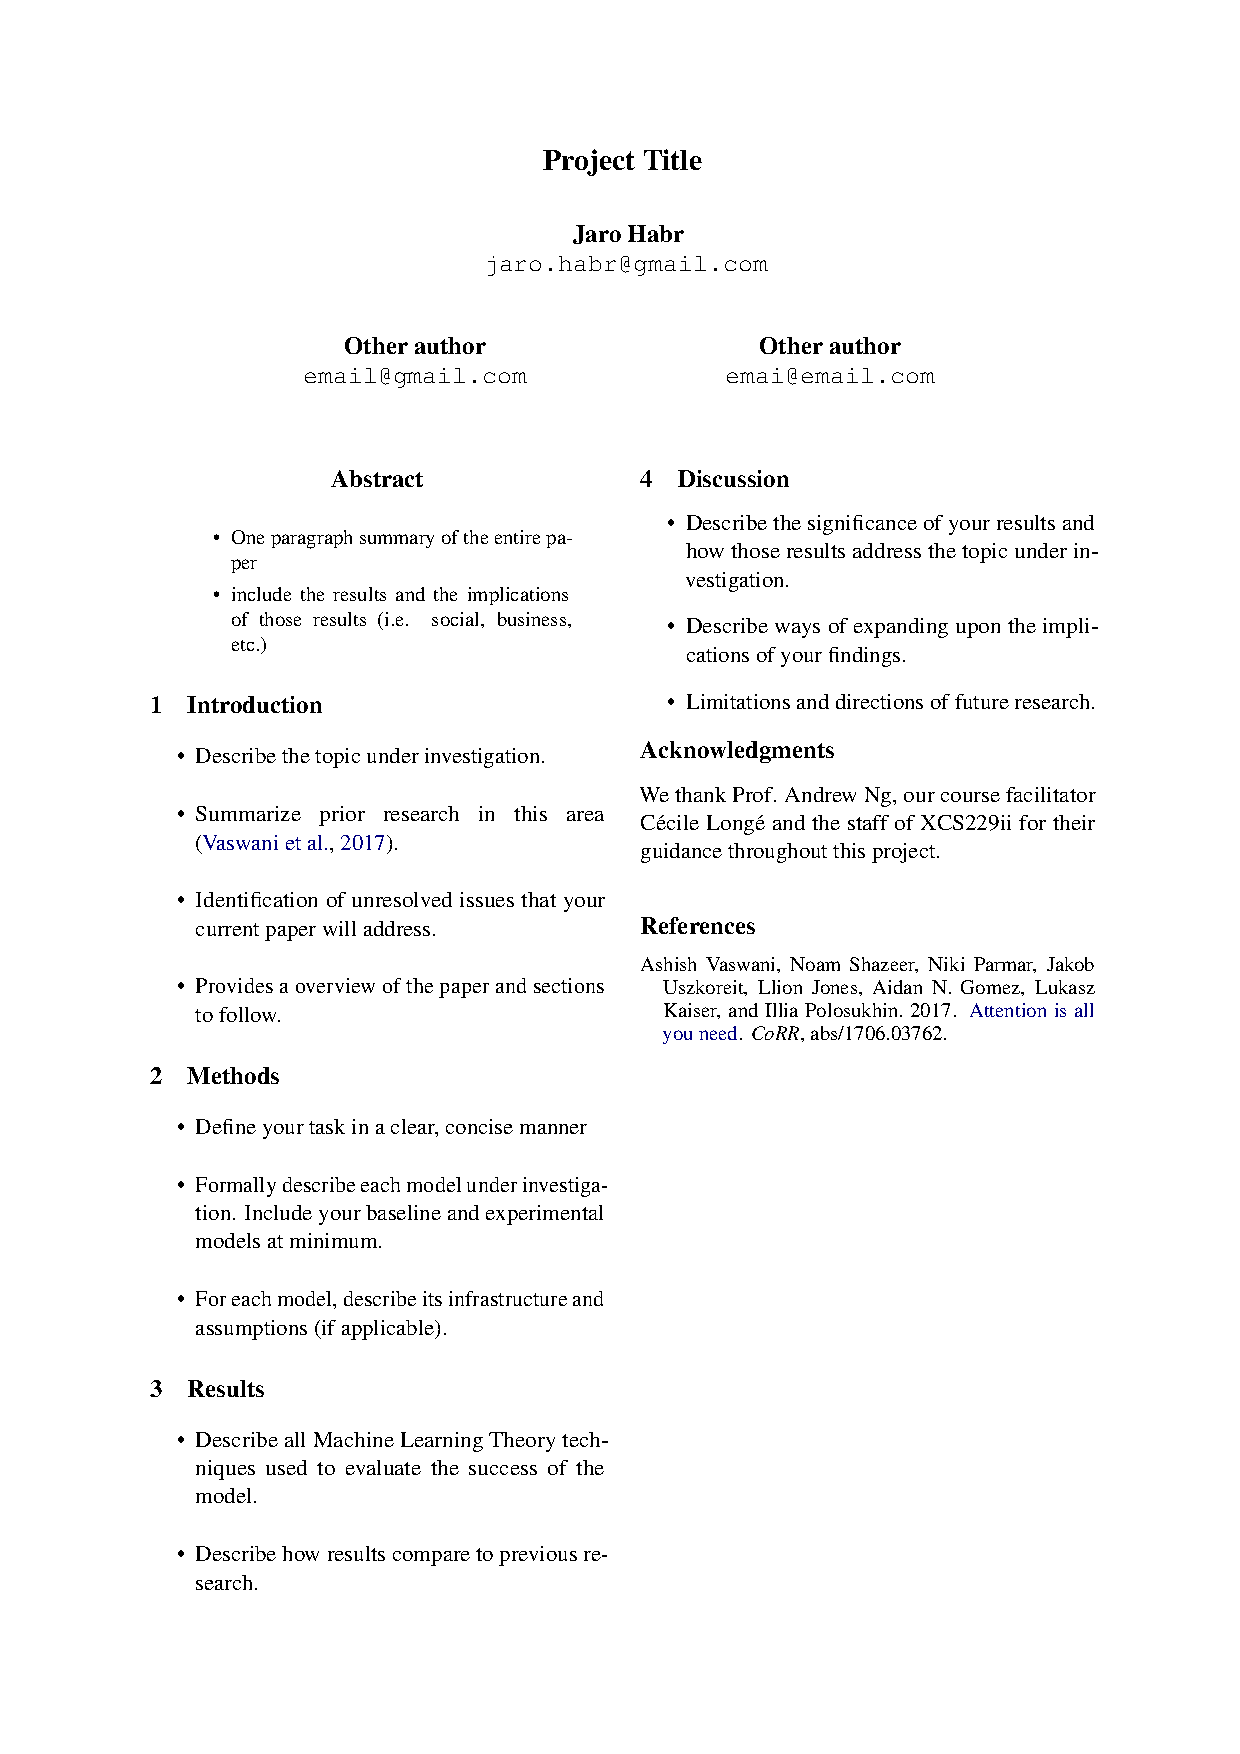
\includegraphics[width=\columnwidth]{assets/figure.pdf}
%   \caption[Caption}
%   \label{figure:4}
% \end{figure}

% \begin{figure}[ht]
%   \centering
%   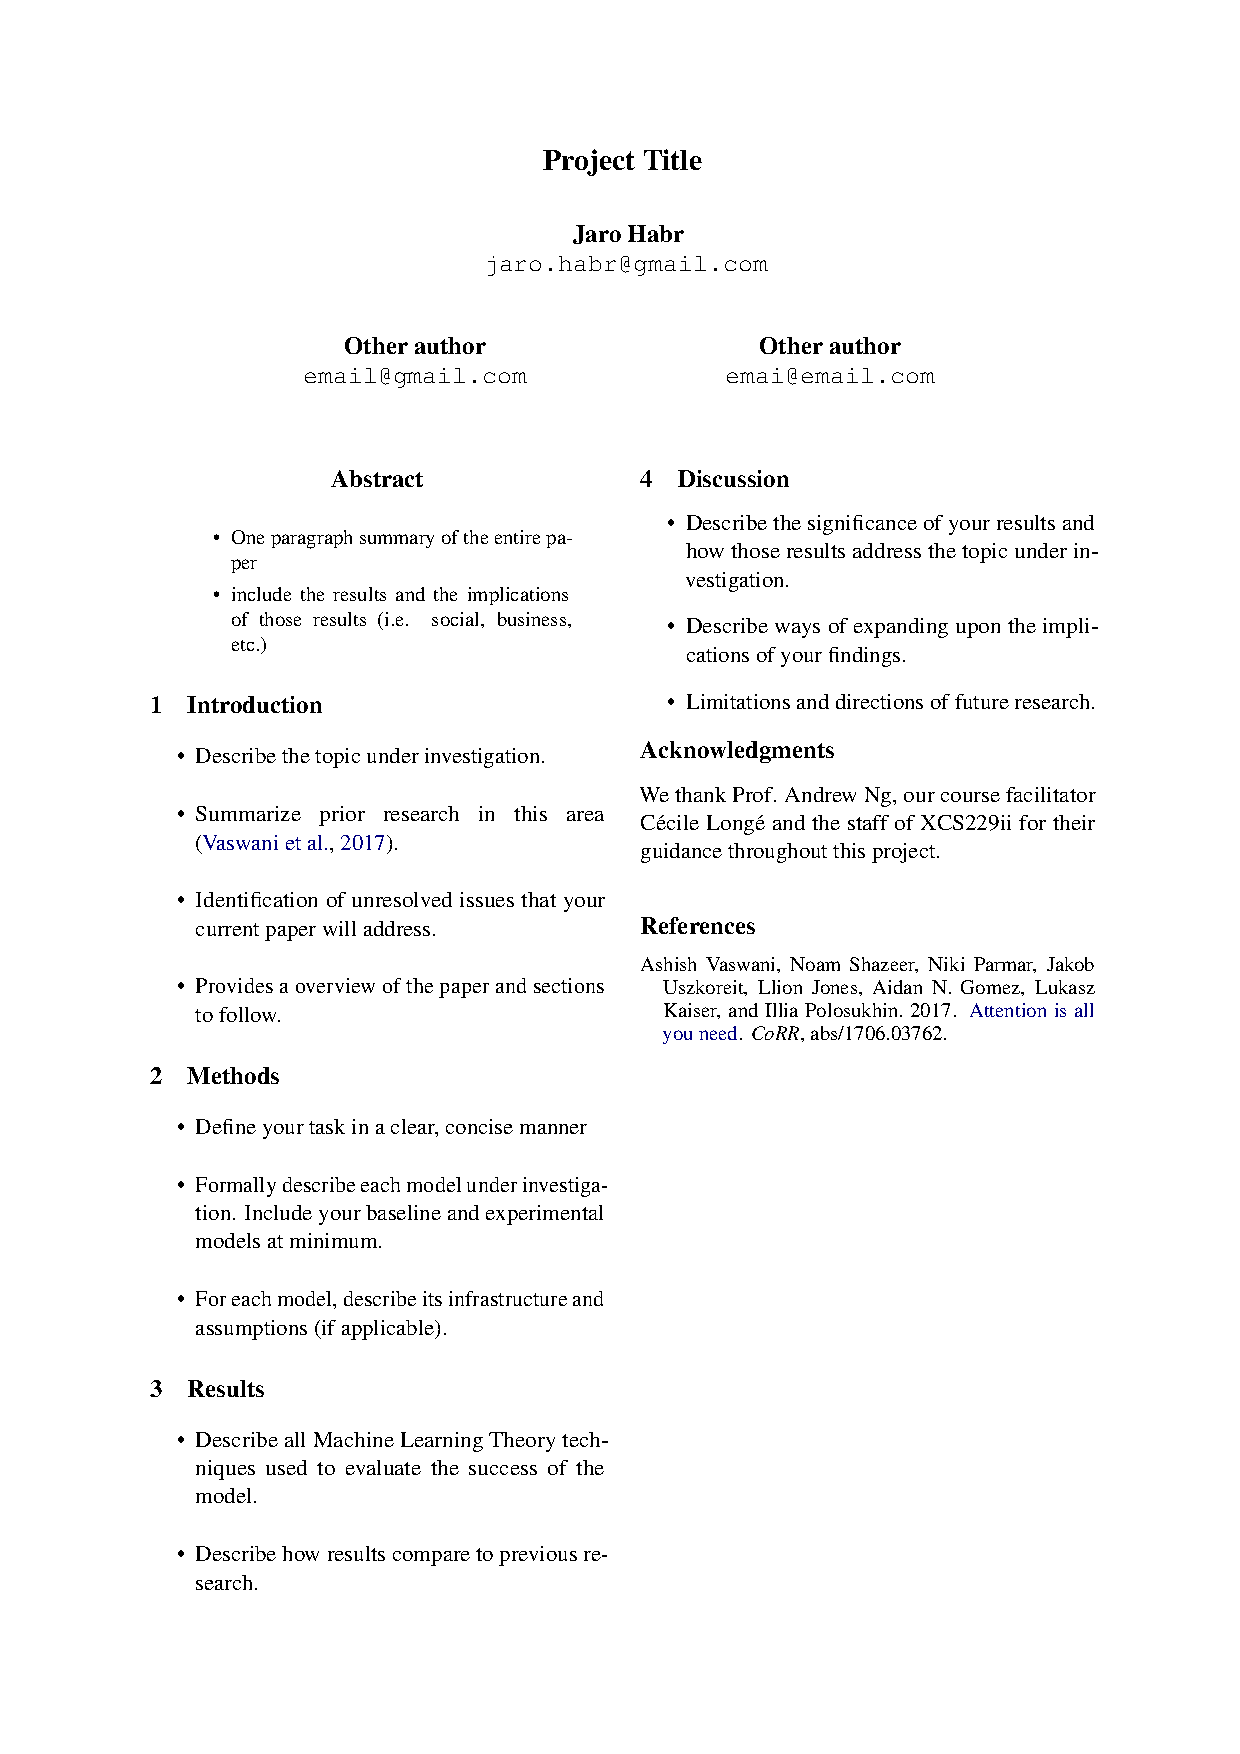
\includegraphics[width=\columnwidth]{assets/figure.pdf}
%   \caption[Caption}
%   \label{figure:5}
% \end{figure}


\end{document}
